\documentclass[]{article}

\usepackage{amsmath}
\DeclareMathOperator{\Lapl}{\mathcal{L}}
\DeclareMathOperator{\bigO}{\mathcal{O}}

\usepackage[bottom]{footmisc}

\usepackage[backend=bibtex, natbib=true, style=numeric, sorting=none]{biblatex}
\addbibresource{bib.bib}

\usepackage{graphicx}

\usepackage{enumitem}

\title{Spectral Graph Theory and High Performance Computing \\ Master Thesis}
\author{David Wobrock\ \texttt{david.wobrock@gmail.com}}

\begin{document}

\begin{titlepage}
 \maketitle
\end{titlepage}

\tableofcontents
\newpage

\section{Image Processing using the Graph Laplacian Operator}

\subsection{Introduction}

The talk by Peyman Milanfar \cite{siam_slides_2016}, working at Google Research, about using the Graph Laplacian Operator for Image Processing purposes awakes curiosity.
% TODO more intro (smartphone, picture, limited resources, performances, Instagram filters)

\subsection{Theory basis}

\paragraph{}
Multiple image processing filters can be built by Graph Laplacians. As Milanfar mentions in \cite{siam_slides_2016}, smoothing, deblurring, sharpening, dehazing, and other filters can be created. Laplacians can also be used for compression artifact removal and low-light imaging.

As it is known, an image filter consists of a function which outputs one pixel, and taking all pixels as input and applying weights to them. We can write this as
\[z_i = \sum_j W_{ij}y_j,\]
\(z_i\) being the output pixel, \(W_{ij}\) the weight and \(y_j\) all input pixels.
This means that we have a vector of weights for each pixel.

So, as a practical notation, we can say that, with \(W\) the matrix of weights and \(y\) the input image as a vector,
\[z = Wy.\]

\paragraph{}
Now we want to represent the image as a graph.
Each pixel is a node and has edges to multiple other nodes.
We can define how the pixels connect to each other, and we can ultimately say that the graph is complete, each node connects to all other nodes.
But we can weigh the edges to measure the similarity between pixels.

\paragraph{}
Affinity, or similarity, is a subjective term which we can also define as we need.
Pixel can be similar if they are spatially close, or if they have the same color, or both for example.
These similarities give us the affinity matrix\footnote{Also called kernel matrix or similarity matrix} called \(K\).

\paragraph{}
By extending this affinity matrix, we obtain the Graph Laplacian \(\Lapl\).
And we want to build this filter \(W\) from the Laplacian.

\paragraph{}
According to \cite{modern_tour_2013}, to build a filter from the Laplacian, we have
\[W = I - \Lapl,\]
and so reciprocally
\[\Lapl = I - W.\]
The Graph Laplacian has multiple definitions, but the simplest is the unnormalised one:
\[\Lapl_U = D - K,\]
with \(D\) a positive definite diagonal matrix with the normalising factors as \(D_{jj} = diag\{\sum_i K_{ij}\}\) along its diagonal.
Other definitions of the Laplacian are shown later in this document. % TODO where? reference to section

\paragraph{}
Interestingly, we can define from \cite{glide_2014} that, by approximating \(W\) by a symmetric, positive definite, double stochastic matrix, this symmetric \(W\) can be computed thanks to this eigen-decomposition
\[W = VSV^T,\]
\(V\) being the eigenvectors and \(S\) the eigenvalues as a diagonal matrix.

Our global filter can be expressed as
\[z = Wy = VSV^Ty.\]

This will be useful since the filter matrix \(W\) becomes huge very quickly and we will need a way to approximate it. Indeed, \(W\) is a square matrix with \(n*n\) elements, \(n\) the number of pixels in the picture.

\paragraph{Approximation by Nystr\"om Extension}

To compute the filter, the first matrix that is needed is the affinity matrix \(K\).
Both matrices have the same size and are computationally expensive.

That is why we approximate the affinity matrix by sampling the picture.
We sample \(p\) pixels, such as  \(p << n\).

Different sampling techniques exist and are shown later in this document. % TODO reference to section

Once sampled, we compute \(K_A\) and \(K_B\), which are parts of \(K\) such as
\[
 K = \begin{bmatrix}
  K_A & K_B \\
  K_B^T & K_C
 \end{bmatrix}.
\]
\(K_A\) represents the affinity matrix of size \(p*p\) between the sample pixels, and \(K_B\) the affinity matrix of size \(p*m\), such as \(m = n-p\), between the sample pixels and the remaining pixels.

These matrices will be computed thanks to a kernel function (or affinity function). This can be the bilateral filter, non-local means or another.

Once computed, we can approximate the eigenvectors \(\Phi\) and eigenvalues \(\Pi\) of \(K\) thanks to the eigen-decomposition of \(K_A\).

As in \cite{glide_2014}, we can define the decomposition of \(K_A\)
\[K_A = \Phi_A \Pi_A \Phi_A^T\]
and the approximation of \(K\) such as
\[\tilde{K} = \tilde{\Phi} \Pi_A \tilde{\Phi}^T\]
and finally the approximation of the \(p\) first eigenvectors of \(K\)
\[
 \tilde{\Phi} = \begin{bmatrix}
  \Phi_A \\
  K_B^T \Phi_A \Pi_A^{-1}
 \end{bmatrix}
\]

From this eigen-decomposition approximation of \(K\), we can then approximate the eigenvectors and eigenvalues of \(W\).
% TODO theory about this

\paragraph{}
One might wonder how an approximation of the first elements of the eigen-decomposition can be enough to approximate the whole matrix.
Indeed, the eigenvalues decay quickly as shown in \cite{siam_slides_2016} and \cite{meyer_perturbation_2014}.

As our experiment below shows, the eigenvalues decay very quickly which means that the whole matrix is mainly defined by the first elements.

% TODO experiment + how is image + explain sampling + kernel method + laplacian


\subsection{First implementation}

\paragraph{Details}
The first implementation of this flow is aimed to denoise the input image.
The sample pixels are selected in a spatially uniform manner.
It uses the NLM from \cite{buades_review_2005} as kernel method to compute the pixels similarity.
The Laplacian matrix is defined through the Sinkhorn iterative algorithm \cite{milanfar_symmetrizing_2013}, where the resulting approximated eigenvectors require to be orthogonalised, which can be done in one step, as discussed in \cite{fowlkes_spectral_2004}.
We finally apply our approximated filter to the noisy image.

The implementation is inspired by the MatLab implementation of \cite{glide_2014}.

\paragraph{Results}
The results of this very first experiment are not yet satisfying as we can observe visually:

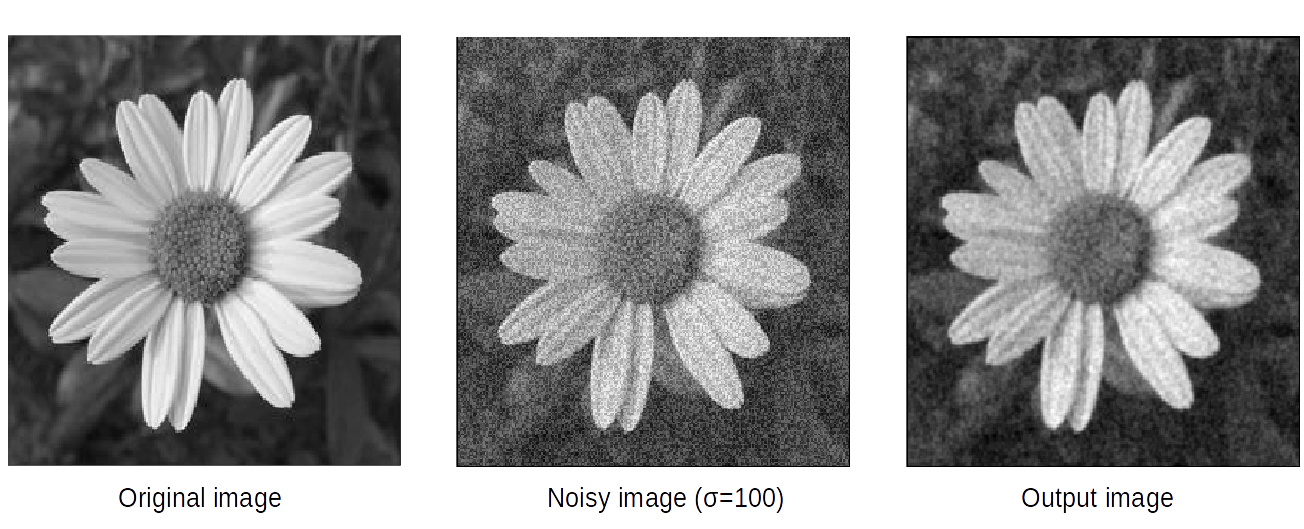
\includegraphics[width=\textwidth]{img/firstimpl.png} % TODO retake this picture maybe

We observe that the output picture is still quite noisy and blurry, we can certainly do better.

\subsection{Algorithm variations}


\subsubsection{Sampling method}
The sample required less than 1\% of the pixels of the image. To achieve this, we can use different approaches. The chosen method is decisive for the Nystr\"om method.
\begin{description}[align=left]
 \item [Random sampling (RS)] most common and simple sampling scheme, but no deterministic guarantee of the output quality. Can produce good results for images with poor resolution, but with a huge amount of data, random sampling is limited because it cannot reflect the structure of the data set \cite{zhan_improved_2017}.
 \item [K-means sampling (KS)] associate to each pixel a 5-D space (R, G, B, X, Y) and divide the pixels into K clusters (K centers). These clusters are a good sampling scheme for images with simple and uniform backgrounds \cite{kao_sampling_2012} \cite{zhang_improved_2008}.
 \item [Uniform spatially sampling] the uniformity of the sample gives good results for image sampling because of the spatial correlation of pixels. This method remains simple but effective \cite{glide_2014}.
 \item [Incremental sampling (INS)] is an adaptive sampling scheme, meaning that it select points according to the similarity, so that we can have an approximate optimal rank-k subspace of the original image \cite{zhan_improved_2017}.
 \item [Mean-shift segmentation-based sampling] this scheme performs good for complex backgrounds. The method consists in over-segmenting the image into \(n\) regions and only one pixel of each region will be sampled using the spatially closest pixel to the center of the region given a formula in \cite{kao_sampling_2012}.
\end{description}

\subsubsection{Affinity function}
The kernel function \(K_{ij}\) measures the similarity between the pixel \(y_i\) and \(y_j\).

\paragraph{Listing}

\begin{description}[align=left]
 \item [Spatial Gaussian Kernel] takes into account only the spatial distance between two pixels \cite{siam_slides_2016}.
 \item [Photometric Gaussian Kernel] considers the intensity and color similarity of the pixels \cite{siam_slides_2016}.
 \item [Bilateral Kernel] one of the most used kernel which smooths images by a nonlinear combination of the spatial and photometric gaussian kernels \cite{siam_slides_2016} \cite{glide_2014}.
 \item [Non-Local Means (NLM)] is similar to the bilateral kernel, a data-dependent filter, except that the photometric affinity is captured patch-wise \cite{glide_2014}.
 %\item [LARK] uses the geodesic distance based on estimated gradients. TODO need more reliable source
\end{description}

\paragraph{Examples}

To illustrate the impact of the affinity function, here are some examples of the affinity matrix for certain pixels.
The more a pixel is colored in red, the more similar it is to the selected pixel, with respect to the chosen function.
A blue colored pixel is dissimilar to the considered pixel.

% TODO include 2 images with NLM function

% TODO include 2 images with spatial function

% TODO 2 images with bilateral function

\subsubsection{Graph Laplacian}
Graph Laplacian has multiple possible definitions and each has its own properties.
A good summary can be found in \cite{siam_slides_2016}.
A Graph Laplacian can be symmetric which is important for eigen-decomposition of the matrix.
It can have a DC eigenvector, which means that the Laplacian has to give 0 if we apply it to a constant image. This is also useful to have.
And the spectral range, corresponding to the range of the eigenvalues, is important because we will use the filters derived from the Laplacian multiple times, and if the eigenvalues are not between 0 and 1, then the filters tend to be unstable.
With \(K\) being the affinity matrix, \(d_i = \sum_j K_{ij}\) and \(D = diag{d_i}^n_1\):

\begin{table}
 \centering
 \begin{tabular}{|c|c|c|c|c|}
  \hline
  Laplacian Name & Formula & Symmetric & DC eigenvector & Spectral Range \\
  \hline
  Un-normalised & \(D - K\) & Yes & Yes & [0, n] \\
  \hline
  Normalised & \(I - D^{-1/2}KD^{-1/2}\) & Yes & No & [0, 2] \\
  \hline
  Random Walk & \(I - D^{-1}K\) & No & Yes & [0, 1] \\
  \hline
  ``Sinkhorn" \cite{milanfar_symmetrizing_2013} & \(I - C^{-1/2}KC^{-1/2}\) & Yes & Yes & [0, 1] \\
  \hline
  Re-normalised & \(\alpha(D - K)\), \(\alpha = \bigO(n^{-1})\) & Yes & Yes & [0, 1] \\
  \hline
 \end{tabular}
\end{table}

Generally, it is a good practice to stick to one definition of the Laplacian.

\clearpage
\printbibliography

\end{document}
